\chapter{Overgangsmetalen en coördinatieverbindingen}\label{ch:b2:coordination-complexes}

In 1893 nam een scheikundige van zesentwintig, Alfred Werner, zich voor een raadsel op te lossen.
Kobalt(III)chloride vormt met ammoniak vier verbindingen, \ce{CoCl3.6NH3},
\ce{CoCl3.5NH3} en twee met de formule \ce{CoCl3.4NH3}, de ene groen en de andere violet.
Zilvernitraat slaat bij de eerste alle drie chloriden meteen neer, bij de
tweede twee, en bij elk van de laatste twee slechts één. Het antwoord van Werner --- zes
groepen die op de hoekpunten van een octaëder rond het metaal gehouden worden, de rest erbuiten
--- legde de grondslag van de coördinatiechemie. Dit hoofdstuk breidt de complexen van het
deel van jaar~1 uit met hun geometrie, hun isomeren, hun namen, en een telling van
elektronen die voorspelt welke metaalcarbonylen bestaan.

\begin{recall}
Het deel van jaar~1: complex, centraal atoom, ligand, meertandig ligand, chelaat,
vormingsconstanten, coördinatiegetal; elektronenconfiguraties van de
ionen van de overgangsmetalen (de $n$s-elektronen gaan eerst verloren); lewiszuren en -basen,
datieve bindingen; VSEPR; oxidatiegetallen; enantiomeren. \Cref{ch:b2:atomic-orbitals}:
de d-orbitalen en de volgorde van de 4s- en 3d-niveaus.
\end{recall}

\begin{omfigure}
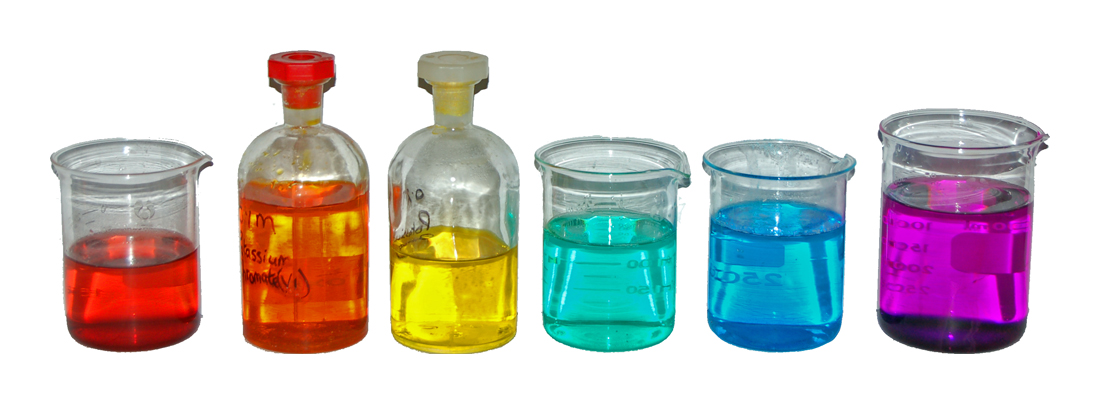
\includegraphics[width=0.8\linewidth]{images/book3/tm-solutions.jpg}

{\small Waterige oplossingen van verbindingen van overgangsmetalen: van links naar rechts
kobalt(II)nitraat, kaliumdichromaat, kaliumchromaat, nikkel(II)chloride,
koper(II)sulfaat en kaliumpermanganaat. De kleuren van de oplossingen van kobalt, nikkel
en koper komen van hun aquacomplexen. (Foto: Benjah-bmm27,
publiek domein, Wikimedia Commons.)}
\end{omfigure}

\section{Het d-blok}

\begin{definition}[Overgangselement]\label{def:b2:coordination-complexes:transition-element}
Een \emph{overgangselement}\index{overgangselement} is een element waarvan het atoom, of
een van de gangbare ionen, een gedeeltelijk gevulde d-subschil heeft. Een ion van zo'n element
met $n$ elektronen in zijn d-orbitalen heeft een \emph{$d^n$-configuratie}\index{dn-configuratie@$d^n$-configuratie}.
\end{definition}

\begin{proposition}[d-elektronen tellen]\label{prop:b2:coordination-complexes:dn}
Een ion $\mathrm M^{m+}$ van een overgangsmetaal uit de groep met nummer $g$ (3 tot 12) heeft een
$d^n$-configuratie met $n = g - m$.
\end{proposition}

\begin{proof}
Het neutrale atoom heeft $g$ elektronen voorbij het voorafgaande edelgas, in de $n$s- en
$(n - 1)$d-orbitalen. In de ionen liggen de d-orbitalen onder de s-orbitaal
(\cref{ex:b2:atomic-orbitals:iron}): alle $g - m$ overblijvende valentie-elektronen zijn
d-elektronen.
\end{proof}

Zo is \ce{Fe^2+} (groep 8) $d^6$, \ce{Cu^2+} (groep 11) $d^9$, \ce{Co^3+} (groep 9)
$d^6$, \ce{Pt^2+} (groep 10) $d^8$.

\section{Liganden}

\begin{definition}[Tandigheid]\label{def:b2:coordination-complexes:denticity}
De \emph{tandigheid}\index{tandigheid} van een ligand is het aantal van zijn atomen dat aan
hetzelfde centrale atoom gebonden is. Een \emph{eentandig ligand}\index{eentandig ligand} bindt
via één atoom (\ce{H2O}, \ce{NH3}, \ce{Cl-}, \ce{CO}), een \emph{tweetandig
ligand}\index{tweetandig ligand} via twee (ethaan-1,2-diamine, geschreven als en; het
ethaandioaation, ox). Een \emph{brugligand}\index{brugligand} bindt tegelijk aan twee
metaalatomen. Een \emph{ambidentaat ligand}\index{ambidentaat ligand} kan binden
via het ene of het andere van twee verschillende atomen, zoals het nitrietion (via N of O) of
thiocyanaat (via S of N).
\end{definition}

\begin{definition}[Coördinatiesfeer]\label{def:b2:coordination-complexes:coordination-sphere}
De \emph{coördinatiesfeer}\index{coordinatiesfeer@coördinatiesfeer} van een complex is het geheel van
het centrale atoom en de liganden die eraan gebonden zijn, geschreven tussen vierkante haken; ionen
buiten de haken zijn tegenionen, niet aan het metaal gebonden.
\end{definition}

\begin{omfigure}
\setchemfig{atom sep=2.2em}
\chemfig{M*5(-H_2N-CH_2-CH_2-NH_2-)}
\qquad
\chemfig{M*5(-O-(=O)-(=O)-O-)}
\qquad
\chemfig{N(-[:120]CH_2COO^{-})(-[:240]CH_2COO^{-})-CH_2-CH_2-N(-[:60]CH_2COO^{-})(-[:-60]CH_2COO^{-})}

\medskip
{\small Chelerende liganden. Links: ethaan-1,2-diamine (en), tweetandig via zijn twee
stikstofatomen. Midden: het ethaandioaation (ox), tweetandig via twee zuurstofatomen. Rechts:
het edta-anion, dat zich om een metaalion wikkelt met zijn twee stikstofatomen en vier
carboxylaatzuurstofatomen (zestandig).}
\end{omfigure}

\section{Coördinatiegetallen en geometrieën}

Twee, vier en zes zijn de meest voorkomende coördinatiegetallen. Zilver(I) en goud(I) geven
lineaire complexen (\ce{[Ag(NH3)2]+}); vier liganden vormen een tetraëder
(\ce{[CoCl4]^2-}, \ce{[Zn(NH3)4]^2+}) of een vierkant (\ce{[PtCl4]^2-}, \ce{[Ni(CN)4]^2-});
vijf een trigonale bipiramide (\ce{Fe(CO)5}); zes, verreweg het vaakst, een
octaëder.

\begin{omfigure}
\begin{tikzpicture}[font=\small]
  \node[omligand] at (-0.8,0) {}; \node[omligand] at (0.8,0) {};
  \draw[thick, black!70] (-0.8,0) -- (0.8,0); \node[ommetal] at (0,0) {};
  \node at (0,-1.5) {lineair, 2};
  \pic at (3,0) {omtetrahedron}; \node at (3,-1.5) {tetraëdrisch, 4};
  \pic at (6,0) {omsquareplanar}; \node at (6,-1.5) {vlak vierkant, 4};
  \pic at (9,0) {omtbp}; \node[align=center] at (9,-1.65) {trigonaal\\ bipiramidaal, 5};
  \pic at (12,0) {omoctahedron}; \node at (12,-1.5) {octaëdrisch, 6};
\end{tikzpicture}

{\small De gangbare coördinatiegeometrieën (metaal oranje, liganden grijs; gestreepte
bindingen wijzen achter het blad).}
\end{omfigure}

VSEPR, dat de elektronenparen van het centrale atoom zo ver mogelijk uit elkaar plaatst,
schiet hier tekort: een $d^8$-ion zoals \ce{Pt^2+} draagt vier paren d-elektronen en vier
liganden, en toch zijn zijn complexen vierkant, niet tetraëdrisch of octaëdrisch. De
d-elektronen zijn geen gelokaliseerde paren die de liganden wegduwen: hun energieën hangen
af van de geometrie op een manier die het volgende hoofdstuk berekent.

\begin{proposition}[Vlak vierkante $d^8$-complexen]\label{prop:b2:coordination-complexes:square-planar}
Complexen met coördinatiegetal vier van $d^8$-ionen van de tweede en derde overgangsreeks
(\ce{Pd^2+}, \ce{Pt^2+}, \ce{Au^3+}) zijn vlak vierkant.
\end{proposition}

\admitted

De verklaring, de splitsing van de d-niveaus door de liganden, komt in
\cref{ch:b2:ligand-field}.

\section{Isomeren}

\begin{definition}[Isomeren van complexen]\label{def:b2:coordination-complexes:isomers}
In een octaëdrisch complex $\mathrm{MA_3B_3}$ heeft het \emph{fac-isomeer}\index{fac-isomeer}
de drie liganden B op één vlak van de octaëder, het \emph{mer-isomeer}\index{mer-isomeer}
op een meridiaan (drie posities in een vlak door het
metaal). \emph{Bindingsisomeren}\index{bindingsisomeren} verschillen in het atoom waarmee
een \omterm{def:b2:coordination-complexes:denticity}{ambidentaat ligand} bindt. \emph{Ionisatie-isomeren}\index{ionisatie-isomeren}
verwisselen een ligand met een tegenion, wat in oplossing verschillende ionen geeft.
\end{definition}

\begin{proposition}[Octaëdrische isomeren tellen]\label{prop:b2:coordination-complexes:isomer-count}
In een octaëder heeft $\mathrm{MA_4B_2}$ twee isomeren (cis en trans), $\mathrm{MA_3B_3}$ twee
(fac en mer), en $\mathrm M(\mathrm{AA})_3$, met drie tweetandige liganden, twee
enantiomeren, $\Delta$ en $\Lambda$.
\end{proposition}

\begin{proof}
In een octaëder zijn twee posities ofwel naburig (cis, $90^\circ$) ofwel tegenover elkaar
(trans, $180^\circ$): twee schikkingen voor de twee liganden B. Voor drie liganden B
staan er ofwel geen twee trans (ze bezetten één vlak: fac) ofwel precies één paar trans (het
derde staat cis ten opzichte van beide: mer); drie onderling trans staande posities bestaan niet. Voor
$\mathrm M(\mathrm{AA})_3$ overspant elk chelaat twee cisposities; de drie chelaten
winden zich om de drietallige as als de bladen van een schroef, met de wijzers van de klok mee
of ertegenin, gezien langs die as: twee spiegelbeelden, die niet samenvallen,
omdat het complex geen spiegelvlak heeft.
\end{proof}

\begin{omfigure}
\begin{tikzpicture}[font=\scriptsize]
  \pic (a) at (0,0) {omoctahedron};
  \node[omligand, fill=omDef!70] at (a-L1) {}; \node[omligand, fill=omDef!70] at (a-L3) {};
  \node at (0,-1.5) {\small cis-$\mathrm{MA_4B_2}$};
  \pic (b) at (3,0) {omoctahedron};
  \node[omligand, fill=omDef!70] at (b-L1) {}; \node[omligand, fill=omDef!70] at (b-L2) {};
  \node at (3,-1.5) {\small trans-$\mathrm{MA_4B_2}$};
  \pic (c) at (6.5,0) {omoctahedron};
  \node[omligand, fill=omThm!70] at (c-L1) {}; \node[omligand, fill=omThm!70] at (c-L3) {}; \node[omligand, fill=omThm!70] at (c-L5) {};
  \node at (6.5,-1.5) {\small fac-$\mathrm{MA_3B_3}$};
  \pic (d) at (9.5,0) {omoctahedron};
  \node[omligand, fill=omThm!70] at (d-L1) {}; \node[omligand, fill=omThm!70] at (d-L2) {}; \node[omligand, fill=omThm!70] at (d-L3) {};
  \node at (9.5,-1.5) {\small mer-$\mathrm{MA_3B_3}$};
\end{tikzpicture}

\medskip
\begin{tikzpicture}[font=\scriptsize]
  \foreach \xs/\s/\lab in {0/1/{$\Delta$}, 4.5/-1/{$\Lambda$}} {
    \begin{scope}[xshift=\xs cm, xscale=\s]
      \draw[black!30] (0,0) circle (1.2);
      \foreach \a in {90, 210, 330} {
        \coordinate (p) at (\a:1.1); \coordinate (q) at (\a+70:0.55);
        \draw[very thick, omDef] (\a:1.1) .. controls (\a+30:1.25) and (\a+60:0.9) .. (\a+75:0.55);
        \node[omligand] at (\a:1.1) {}; \node[omligand] at (\a+75:0.55) {};
      }
      \node[ommetal] at (0,0) {};
    \end{scope}
    \node at (\xs,-1.6) {\small \lab};
  }
  \draw[densely dashed] (2.25,-1.3) -- (2.25,1.3);
  \node[anchor=south] at (2.25,1.3) {spiegel};
\end{tikzpicture}

{\small Boven: cis- en trans-isomeren van $\mathrm{MA_4B_2}$ (liganden B blauw), fac- en mer-isomeren
van $\mathrm{MA_3B_3}$ (B rood). Onder: de twee enantiomeren van een trischelaat zoals
\ce{[Co(en)3]^3+}, gezien langs de drietallige as, schematisch: elk chelaat (blauwe
boog) verbindt een bovenste en een onderste positie, en de drie draaien in de ene richting ($\Delta$) of
in de andere ($\Lambda$).}
\end{omfigure}

\section{Namen en elektronentellingen}

\begin{method}[Een complex benoemen]\label{met:b2:coordination-complexes:naming}
\begin{enumerate}
  \item Schrijf in de formule de \omterm{def:b2:coordination-complexes:coordination-sphere}{coördinatiesfeer} tussen vierkante haken, het metaal
        eerst, dan de liganden; de lading van het complex erbuiten.
  \item Som in de naam de liganden in alfabetische volgorde op, met vermenigvuldigende
        voorvoegsels (di-, tri-, tetra-; bis-, tris- voor samengestelde ligandnamen): anionische
        liganden eindigen op -o (chlorido, cyanido, oxido, hydroxido), neutrale behouden
        hun naam (aqua, ammine, carbonyl).
  \item Dan het metaal, met de uitgang -aat als het complex een anion is (ferraat,
        cupraat, kobaltaat), en zijn oxidatiegetal in Romeinse cijfers.
  \item Kationen worden vóór anionen genoemd: \ce{[Co(NH3)6]Cl3} is
        hexaamminekobalt(III)chloride, \ce{K4[Fe(CN)6]}
        kaliumhexacyanidoferraat(II).
\end{enumerate}
\end{method}

\begin{definition}[Elektronentelling]\label{def:b2:coordination-complexes:electron-count}
De \emph{valentie-elektronentelling}\index{valentie-elektronentelling} van een complex is het
aantal d-elektronen van het metaalion plus de elektronen die de liganden leveren (twee
voor elk donorpaar). De \emph{18-elektronenregel}\index{18-elektronenregel} zegt dat
stabiele complexen van metalen in een lage oxidatietoestand met sterk bindende $\pi$-acceptorliganden
zoals \ce{CO} doorgaans 18 valentie-elektronen hebben.
\end{definition}

\begin{definition}[Hapticiteit]\label{def:b2:coordination-complexes:hapticity}
De \emph{hapticiteit}\index{hapticiteit} van een ligand is het aantal van zijn atomen dat
via één doorlopend $\pi$-systeem aan het metaal gebonden is; ze wordt geschreven als $\eta^n$: een etheen dat via
zijn $\pi$-binding gebonden is, is $\eta^2$, een cyclopentadienylring die via alle vijf koolstofatomen gebonden is, $\eta^5$.
\end{definition}

\begin{method}[Elektronen tellen]\label{met:b2:coordination-complexes:electron-count}
\begin{enumerate}
  \item Geef de liganden ladingen als deeltjes met gesloten schil (\ce{Cl-}, \ce{H-},
        \ce{C5H5-}; \ce{CO}, \ce{PR3}, \ce{NH3} neutraal) en leid de oxidatietoestand
        van het metaal af.
  \item Tel de d-elektronen van het metaal, $n = g - m$.
  \item Tel twee elektronen op per donorpaar: één paar per \omterm{def:b2:coordination-complexes:denticity}{eentandig ligand}, zes voor een
        $\eta^5$-\ce{C5H5-}, zes voor een $\eta^6$-benzeen, twee voor een $\eta^2$-alkeen.
  \item Een metaal-metaalbinding telt één elektron voor elk metaal.
\end{enumerate}
\end{method}

\begin{proposition}[Metaalcarbonylen]\label{prop:b2:coordination-complexes:eighteen}
De stabiele binaire carbonylen van de eerste overgangsreeks, \ce{Cr(CO)6},
\ce{Fe(CO)5}, \ce{Ni(CO)4} en \ce{Mn2(CO)10}, hebben alle 18 valentie-elektronen per
metaalatoom.
\end{proposition}

\begin{proof}
Chroom(0), $d^6$, met zes CO: $6 + 12 = 18$. IJzer(0), $d^8$, vijf CO: $8 + 10 = 18$.
Nikkel(0), $d^{10}$, vier CO: $10 + 8 = 18$. Mangaan(0), $d^7$, vijf CO en één
binding Mn--Mn: $7 + 10 + 1 = 18$; een monomeer \ce{Mn(CO)5}, met 17, bestaat niet als
stabiele verbinding, en vormt een paar. De reden waarom 18 begunstigd is --- negen valentieorbitalen
van het metaal, alle bindende of niet-bindende gevuld --- wordt gegeven in
\cref{ch:b2:ligand-field}.
\end{proof}

Ferroceen, \ce{Fe(\eta^5-C5H5)2}, bevat een ijzer(II)-ion ($d^6$) tussen twee
cyclopentadienylanionen, die elk zes elektronen leveren: $6 + 12 = 18$. De regel faalt voor
de meeste complexen met hoge oxidatietoestanden en voor veel met zwakke liganden: \ce{[Ti(H2O)6]^3+}
heeft 13 elektronen, \ce{[Cu(H2O)6]^2+} 21.

\begin{history}[Werner en de octaëder]
\begin{minipage}[t]{0.22\linewidth}
\vspace{0pt}
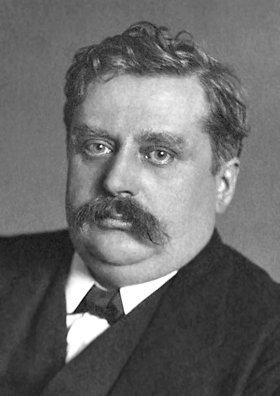
\includegraphics[width=\linewidth]{images/book3/werner.jpg}
\end{minipage}\hfill
\begin{minipage}[t]{0.74\linewidth}
\vspace{0pt}
Alfred Werner stelde in 1893 voor dat een metaal, naast zijn valentie, een
coördinatiegetal heeft van groepen die rechtstreeks eromheen vastgehouden worden, en dat kobalt(III)
er zes vasthoudt op de hoekpunten van een octaëder. Hij voorspelde daarna hoeveel isomeren elke
formule zou moeten hebben en besteedde twintig jaar aan hun bereiding; in 1911 splitste hij een
kobaltcomplex in zijn twee enantiomeren, wat bewees dat chiraliteit geen
koolstofatoom vereist. Hij kreeg in 1913 de Nobelprijs voor Scheikunde. (Portret, Les Prix
Nobel, 1914, publiek domein, Wikimedia Commons.)
\end{minipage}
\end{history}

\section{Oefeningen}

\begin{exercise}[$\star$]\label{exo:b2:coordination-complexes:1}
Geef de $d^n$-configuratie van \ce{Ti^3+}, \ce{V^3+}, \ce{Cr^3+}, \ce{Mn^2+}, \ce{Fe^3+},
\ce{Co^2+}, \ce{Ni^2+} en \ce{Zn^2+}.
\end{exercise}

\begin{exercise}[$\star$]\label{exo:b2:coordination-complexes:2}
Geef de \omterm{def:b2:coordination-complexes:denticity}{tandigheid} van water, ethaan-1,2-diamine, het ethaandioaation, edta en het
thiocyanaation, en zeg welk ligand ambidentaat is.
\end{exercise}

\begin{exercise}[$\star$]\label{exo:b2:coordination-complexes:3}
Benoem \ce{[Cu(NH3)4]SO4}, \ce{K3[Fe(CN)6]}, \ce{[CoCl2(NH3)4]Cl} en
\ce{[Ni(CO)4]}.
\end{exercise}

\begin{exercise}[$\star$]\label{exo:b2:coordination-complexes:4}
Voorspel de geometrie van \ce{[Ag(NH3)2]+}, \ce{[CoCl4]^2-}, \ce{[PtCl4]^2-} en
\ce{[Fe(H2O)6]^2+}.
\end{exercise}

\begin{exercise}[$\star\star$]\label{exo:b2:coordination-complexes:5}
Hoeveel isomeren heeft het vlak vierkante \ce{[PtCl2(NH3)2]}? Teken ze. (Een ervan,
cisplatine, is een geneesmiddel tegen kanker.)
\end{exercise}

\begin{exercise}[$\star\star$]\label{exo:b2:coordination-complexes:6}
Tel de valentie-elektronen van \ce{Cr(CO)6}, \ce{Fe(CO)5}, \ce{Ni(CO)4},
\ce{V(CO)6} en \ce{Mn2(CO)10}. Welke verbinding overtreedt de regel, en hoe gedraagt ze zich?
\end{exercise}

\begin{exercise}[$\star\star$]\label{exo:b2:coordination-complexes:7}
Tel de valentie-elektronen van ferroceen en van kobaltoceen \ce{Co(C5H5)2}. Welke wordt
gemakkelijk geoxideerd, en waartoe?
\end{exercise}

\begin{exercise}[$\star\star$]\label{exo:b2:coordination-complexes:8}
Het nikkel(II)complex van edta heeft $\log_{10}K = 20.5$, ver boven die van complexen waarin
nikkel zes afzonderlijke stikstof- of zuurstofdonoren bindt. Verklaar dit chelaateffect
aan de hand van het aantal deeltjes dat vrijkomt wanneer het chelaat zes watermoleculen
vervangt.
% ledger: logb:Ni-edta
\end{exercise}

\begin{exercise}[$\star\star$]\label{exo:b2:coordination-complexes:9}
Teken de twee \omterm{def:b2:coordination-complexes:isomers}{bindingsisomeren} van \ce{[Co(NO2)(NH3)5]^2+}.
\end{exercise}

\begin{exercise}[$\star\star\star$]\label{exo:b2:coordination-complexes:10}
Hoeveel stereo-isomeren heeft \ce{[CoCl2(en)2]+}? Welke zijn chiraal?
\end{exercise}

\begin{exercise}[$\star\star\star$]\label{exo:b2:coordination-complexes:11}
Tel voor $\mathrm{MA_4B_2}$ de isomeren die voorspeld worden door een vlakke zeshoek en door een trigonaal
prisma van zes liganden, en leg uit hoe het aantal gevonden isomeren tussen de
geometrieën beslist.
\end{exercise}

\begin{exercise}[$\star\star\star$]\label{exo:b2:coordination-complexes:12}
Tel de valentie-elektronen van \ce{[RhCl(PPh3)3]} en van \ce{[IrH(CO)(PPh3)3]}
(\ce{PPh3} een donor van twee elektronen, \ce{H-} als hydride). Welke zou er nog twee
liganden bij kunnen opnemen?
\end{exercise}

\section{Probleem: de kobaltammines van Werner}

\begin{problem}[{Weekendprobleem --- vier ammines van kobalt(III)chloride en het chloride
dat ze vrijgeven, hun formules met haken, de twee isomeren van het tetraammine en wat
ze over de geometrie bewijzen, en de optische activiteit van een trischelaat}]
\label{pb:b2:coordination-complexes:1}
Gegevens: vier verbindingen A \ce{CoCl3.6NH3} (oranjegeel), B \ce{CoCl3.5NH3}
(paars), C en D \ce{CoCl3.4NH3} (groen en violet). Met overmaat zilvernitraat
slaat één mol A 3 mol \ce{AgCl} neer, B 2 mol, C en D elk 1 mol. Molaire
geleidbaarheden tonen 4, 3, 2 en 2 ionen per formule-eenheid.

\medskip
\noindent\textbf{Deel I --- Chloride en ionen.}
\begin{enumerate}
  \item Welke chloriden reageren meteen met zilverionen?
  \item Hoeveel chloriden zijn in elke verbinding aan kobalt gebonden?
  \item Controleer de aantallen ionen aan de hand van de geleidbaarheden.
  \item Wat is het oxidatiegetal van kobalt in alle vier?
  \item Wat is zijn $d^n$-configuratie?
  \item Hoeveel liganden in totaal houdt kobalt in elke verbinding vast?
\end{enumerate}

\medskip
\noindent\textbf{Deel II --- Formules en namen.}
\begin{enumerate}[resume]
  \item Schrijf A, B, C en D met vierkante haken.
  \item Benoem A en B.
  \item Benoem het kation van C en D.
  \item Wat voor isomeren zijn C en D?
  \item Wat zou een verbinding \ce{CoCl3.3NH3} zijn, en hoeveel ionen zou ze geven?
  \item Hoeveel isomeren zou die verbinding in een octaëder hebben?
\end{enumerate}

\medskip
\noindent\textbf{Deel III --- De geometrie.}
\begin{enumerate}[resume]
  \item Teken cis- en trans-\ce{[CoCl2(NH3)4]+} in een octaëder.
  \item Tel de isomeren van \ce{[CoCl2(NH3)4]+} die voorspeld worden voor zes liganden op de
        hoekpunten van een vlakke zeshoek.
  \item Tel die welke voorspeld worden voor een trigonaal prisma.
  \item Werner vond er nooit meer dan twee. Wat bewijst dat?
  \item Is het bewijs volledig? Wat zou een derde isomeer betekend hebben?
  \item Welke van C en D is cis, wetende dat het cis-isomeer met ethaandioaat in een
        chelaat kan worden omgezet en het trans-isomeer niet?
\end{enumerate}

\medskip
\noindent\textbf{Deel IV --- Optische activiteit.}
\begin{enumerate}[resume]
  \item Teken \ce{[Co(en)3]^3+}.
  \item Heeft het een spiegelvlak? Een inversiecentrum?
  \item Hoeveel stereo-isomeren heeft het?
  \item Wat bewijst de splitsing van zo'n kation in enantiomeren?
  \item Is \ce{[CoCl2(en)2]+} chiraal in zijn cisvorm? In zijn transvorm?
  \item Waarom was het belangrijk dat Werner een complex zonder enig koolstofatoom splitste?
  \item Geef het aantal isomeren van \ce{[CoCl2(NH3)4]+} dat voorspeld wordt door de octaëder,
        en door de vlakke zeshoek en het trigonale prisma.
\end{enumerate}
\end{problem}
